\documentclass[twoside]{book}

% Packages required by doxygen
\usepackage{fixltx2e}
\usepackage{calc}
\usepackage{doxygen}
\usepackage[export]{adjustbox} % also loads graphicx
\usepackage{graphicx}
\usepackage[utf8]{inputenc}
\usepackage{makeidx}
\usepackage{multicol}
\usepackage{multirow}
\PassOptionsToPackage{warn}{textcomp}
\usepackage{textcomp}
\usepackage[nointegrals]{wasysym}
\usepackage[table]{xcolor}

% Font selection
\usepackage[T1]{fontenc}
\usepackage[scaled=.90]{helvet}
\usepackage{courier}
\usepackage{amssymb}
\usepackage{sectsty}
\renewcommand{\familydefault}{\sfdefault}
\allsectionsfont{%
  \fontseries{bc}\selectfont%
  \color{darkgray}%
}
\renewcommand{\DoxyLabelFont}{%
  \fontseries{bc}\selectfont%
  \color{darkgray}%
}
\newcommand{\+}{\discretionary{\mbox{\scriptsize$\hookleftarrow$}}{}{}}

% Page & text layout
\usepackage{geometry}
\geometry{%
  a4paper,%
  top=2.5cm,%
  bottom=2.5cm,%
  left=2.5cm,%
  right=2.5cm%
}
\tolerance=750
\hfuzz=15pt
\hbadness=750
\setlength{\emergencystretch}{15pt}
\setlength{\parindent}{0cm}
\setlength{\parskip}{3ex plus 2ex minus 2ex}
\makeatletter
\renewcommand{\paragraph}{%
  \@startsection{paragraph}{4}{0ex}{-1.0ex}{1.0ex}{%
    \normalfont\normalsize\bfseries\SS@parafont%
  }%
}
\renewcommand{\subparagraph}{%
  \@startsection{subparagraph}{5}{0ex}{-1.0ex}{1.0ex}{%
    \normalfont\normalsize\bfseries\SS@subparafont%
  }%
}
\makeatother

% Headers & footers
\usepackage{fancyhdr}
\pagestyle{fancyplain}
\fancyhead[LE]{\fancyplain{}{\bfseries\thepage}}
\fancyhead[CE]{\fancyplain{}{}}
\fancyhead[RE]{\fancyplain{}{\bfseries\leftmark}}
\fancyhead[LO]{\fancyplain{}{\bfseries\rightmark}}
\fancyhead[CO]{\fancyplain{}{}}
\fancyhead[RO]{\fancyplain{}{\bfseries\thepage}}
\fancyfoot[LE]{\fancyplain{}{}}
\fancyfoot[CE]{\fancyplain{}{}}
\fancyfoot[RE]{\fancyplain{}{\bfseries\scriptsize Generated by Doxygen }}
\fancyfoot[LO]{\fancyplain{}{\bfseries\scriptsize Generated by Doxygen }}
\fancyfoot[CO]{\fancyplain{}{}}
\fancyfoot[RO]{\fancyplain{}{}}
\renewcommand{\footrulewidth}{0.4pt}
\renewcommand{\chaptermark}[1]{%
  \markboth{#1}{}%
}
\renewcommand{\sectionmark}[1]{%
  \markright{\thesection\ #1}%
}

% Indices & bibliography
\usepackage{natbib}
\usepackage[titles]{tocloft}
\setcounter{tocdepth}{3}
\setcounter{secnumdepth}{5}
\makeindex

% Hyperlinks (required, but should be loaded last)
\usepackage{ifpdf}
\ifpdf
  \usepackage[pdftex,pagebackref=true]{hyperref}
\else
  \usepackage[ps2pdf,pagebackref=true]{hyperref}
\fi
\hypersetup{%
  colorlinks=true,%
  linkcolor=blue,%
  citecolor=blue,%
  unicode%
}

% Custom commands
\newcommand{\clearemptydoublepage}{%
  \newpage{\pagestyle{empty}\cleardoublepage}%
}

\usepackage{caption}
\captionsetup{labelsep=space,justification=centering,font={bf},singlelinecheck=off,skip=4pt,position=top}

%===== C O N T E N T S =====

\begin{document}

% Titlepage & ToC
\hypersetup{pageanchor=false,
             bookmarksnumbered=true,
             pdfencoding=unicode
            }
\pagenumbering{roman}
\begin{titlepage}
\vspace*{7cm}
\begin{center}%
{\Large Game of Drones Sim }\\
\vspace*{1cm}
{\large Generated by Doxygen 1.8.11}\\
\end{center}
\end{titlepage}
\clearemptydoublepage
\tableofcontents
\clearemptydoublepage
\pagenumbering{arabic}
\hypersetup{pageanchor=true}

%--- Begin generated contents ---
\chapter{Hierarchical Index}
\section{Class Hierarchy}
This inheritance list is sorted roughly, but not completely, alphabetically\+:\begin{DoxyCompactList}
\item \contentsline{section}{Aodv\+\_\+route}{\pageref{class_aodv__route}}{}
\item \contentsline{section}{Comm\+Mod}{\pageref{class_comm_mod}}{}
\begin{DoxyCompactList}
\item \contentsline{section}{Aodv}{\pageref{class_aodv}}{}
\item \contentsline{section}{Basic}{\pageref{class_basic}}{}
\item \contentsline{section}{Basic\+\_\+addressed}{\pageref{class_basic__addressed}}{}
\end{DoxyCompactList}
\item \contentsline{section}{Coord}{\pageref{struct_coord}}{}
\item \contentsline{section}{Environment}{\pageref{class_environment}}{}
\item \contentsline{section}{Ip\+Allocator}{\pageref{class_ip_allocator}}{}
\item \contentsline{section}{Message}{\pageref{class_message}}{}
\begin{DoxyCompactList}
\item \contentsline{section}{Aodv\+\_\+message}{\pageref{class_aodv__message}}{}
\begin{DoxyCompactList}
\item \contentsline{section}{Aodv\+\_\+rerr}{\pageref{class_aodv__rerr}}{}
\item \contentsline{section}{Aodv\+\_\+rrep}{\pageref{class_aodv__rrep}}{}
\item \contentsline{section}{Aodv\+\_\+rreq}{\pageref{class_aodv__rreq}}{}
\end{DoxyCompactList}
\item \contentsline{section}{Basic\+\_\+message}{\pageref{class_basic__message}}{}
\begin{DoxyCompactList}
\item \contentsline{section}{Basic\+\_\+message\+\_\+addressed}{\pageref{class_basic__message__addressed}}{}
\end{DoxyCompactList}
\end{DoxyCompactList}
\item \contentsline{section}{Messageable}{\pageref{class_messageable}}{}
\begin{DoxyCompactList}
\item \contentsline{section}{Base\+Station}{\pageref{class_base_station}}{}
\begin{DoxyCompactList}
\item \contentsline{section}{Sensing\+Base\+Station}{\pageref{class_sensing_base_station}}{}
\end{DoxyCompactList}
\item \contentsline{section}{Drone}{\pageref{class_drone}}{}
\begin{DoxyCompactList}
\item \contentsline{section}{Aodv\+Comms}{\pageref{class_aodv_comms}}{}
\item \contentsline{section}{Sensing\+Drone}{\pageref{class_sensing_drone}}{}
\item \contentsline{section}{Test}{\pageref{class_test}}{}
\item \contentsline{section}{Test}{\pageref{class_test}}{}
\end{DoxyCompactList}
\end{DoxyCompactList}
\end{DoxyCompactList}

\chapter{Class Index}
\section{Class List}
Here are the classes, structs, unions and interfaces with brief descriptions\+:\begin{DoxyCompactList}
\item\contentsline{section}{\hyperlink{class_aodv}{Aodv} }{\pageref{class_aodv}}{}
\item\contentsline{section}{\hyperlink{class_aodv__message}{Aodv\+\_\+message} }{\pageref{class_aodv__message}}{}
\item\contentsline{section}{\hyperlink{class_aodv__rerr}{Aodv\+\_\+rerr} }{\pageref{class_aodv__rerr}}{}
\item\contentsline{section}{\hyperlink{class_aodv__route}{Aodv\+\_\+route} }{\pageref{class_aodv__route}}{}
\item\contentsline{section}{\hyperlink{class_aodv__rrep}{Aodv\+\_\+rrep} }{\pageref{class_aodv__rrep}}{}
\item\contentsline{section}{\hyperlink{class_aodv__rreq}{Aodv\+\_\+rreq} }{\pageref{class_aodv__rreq}}{}
\item\contentsline{section}{\hyperlink{class_aodv_comms}{Aodv\+Comms} }{\pageref{class_aodv_comms}}{}
\item\contentsline{section}{\hyperlink{class_base_station}{Base\+Station} }{\pageref{class_base_station}}{}
\item\contentsline{section}{\hyperlink{class_basic}{Basic} }{\pageref{class_basic}}{}
\item\contentsline{section}{\hyperlink{class_basic__addressed}{Basic\+\_\+addressed} }{\pageref{class_basic__addressed}}{}
\item\contentsline{section}{\hyperlink{class_basic__message}{Basic\+\_\+message} }{\pageref{class_basic__message}}{}
\item\contentsline{section}{\hyperlink{class_basic__message__addressed}{Basic\+\_\+message\+\_\+addressed} }{\pageref{class_basic__message__addressed}}{}
\item\contentsline{section}{\hyperlink{class_comm_mod}{Comm\+Mod} }{\pageref{class_comm_mod}}{}
\item\contentsline{section}{\hyperlink{struct_coord}{Coord} }{\pageref{struct_coord}}{}
\item\contentsline{section}{\hyperlink{class_drone}{Drone} }{\pageref{class_drone}}{}
\item\contentsline{section}{\hyperlink{class_environment}{Environment} }{\pageref{class_environment}}{}
\item\contentsline{section}{\hyperlink{class_ip_allocator}{Ip\+Allocator} }{\pageref{class_ip_allocator}}{}
\item\contentsline{section}{\hyperlink{class_message}{Message} }{\pageref{class_message}}{}
\item\contentsline{section}{\hyperlink{class_messageable}{Messageable} }{\pageref{class_messageable}}{}
\item\contentsline{section}{\hyperlink{class_sensing_base_station}{Sensing\+Base\+Station} }{\pageref{class_sensing_base_station}}{}
\item\contentsline{section}{\hyperlink{class_sensing_drone}{Sensing\+Drone} }{\pageref{class_sensing_drone}}{}
\item\contentsline{section}{\hyperlink{class_test}{Test} }{\pageref{class_test}}{}
\end{DoxyCompactList}

\chapter{File Index}
\section{File List}
Here is a list of all files with brief descriptions\+:\begin{DoxyCompactList}
\item\contentsline{section}{/home/will/\+Documents/effacious-\/octo-\/weasel/code/communication/aodv/\hyperlink{_aodv_8cpp}{Aodv.\+cpp} }{\pageref{_aodv_8cpp}}{}
\item\contentsline{section}{/home/will/\+Documents/effacious-\/octo-\/weasel/code/communication/aodv/\hyperlink{_aodv_8hpp}{Aodv.\+hpp} }{\pageref{_aodv_8hpp}}{}
\item\contentsline{section}{/home/will/\+Documents/effacious-\/octo-\/weasel/code/communication/aodv/\hyperlink{_aodv__message_8cpp}{Aodv\+\_\+message.\+cpp} }{\pageref{_aodv__message_8cpp}}{}
\item\contentsline{section}{/home/will/\+Documents/effacious-\/octo-\/weasel/code/communication/aodv/\hyperlink{_aodv__message_8hpp}{Aodv\+\_\+message.\+hpp} }{\pageref{_aodv__message_8hpp}}{}
\item\contentsline{section}{/home/will/\+Documents/effacious-\/octo-\/weasel/code/communication/aodv/\hyperlink{_aodv__rerr_8cpp}{Aodv\+\_\+rerr.\+cpp} }{\pageref{_aodv__rerr_8cpp}}{}
\item\contentsline{section}{/home/will/\+Documents/effacious-\/octo-\/weasel/code/communication/aodv/\hyperlink{_aodv__rerr_8hpp}{Aodv\+\_\+rerr.\+hpp} }{\pageref{_aodv__rerr_8hpp}}{}
\item\contentsline{section}{/home/will/\+Documents/effacious-\/octo-\/weasel/code/communication/aodv/\hyperlink{_aodv__route_8cpp}{Aodv\+\_\+route.\+cpp} }{\pageref{_aodv__route_8cpp}}{}
\item\contentsline{section}{/home/will/\+Documents/effacious-\/octo-\/weasel/code/communication/aodv/\hyperlink{_aodv__route_8hpp}{Aodv\+\_\+route.\+hpp} }{\pageref{_aodv__route_8hpp}}{}
\item\contentsline{section}{/home/will/\+Documents/effacious-\/octo-\/weasel/code/communication/aodv/\hyperlink{_aodv__rrep_8cpp}{Aodv\+\_\+rrep.\+cpp} }{\pageref{_aodv__rrep_8cpp}}{}
\item\contentsline{section}{/home/will/\+Documents/effacious-\/octo-\/weasel/code/communication/aodv/\hyperlink{_aodv__rrep_8hpp}{Aodv\+\_\+rrep.\+hpp} }{\pageref{_aodv__rrep_8hpp}}{}
\item\contentsline{section}{/home/will/\+Documents/effacious-\/octo-\/weasel/code/communication/aodv/\hyperlink{_aodv__rreq_8cpp}{Aodv\+\_\+rreq.\+cpp} }{\pageref{_aodv__rreq_8cpp}}{}
\item\contentsline{section}{/home/will/\+Documents/effacious-\/octo-\/weasel/code/communication/aodv/\hyperlink{_aodv__rreq_8hpp}{Aodv\+\_\+rreq.\+hpp} }{\pageref{_aodv__rreq_8hpp}}{}
\item\contentsline{section}{/home/will/\+Documents/effacious-\/octo-\/weasel/code/communication/basic/\hyperlink{_basic_8cpp}{Basic.\+cpp} }{\pageref{_basic_8cpp}}{}
\item\contentsline{section}{/home/will/\+Documents/effacious-\/octo-\/weasel/code/communication/basic/\hyperlink{_basic_8hpp}{Basic.\+hpp} }{\pageref{_basic_8hpp}}{}
\item\contentsline{section}{/home/will/\+Documents/effacious-\/octo-\/weasel/code/communication/basic/\hyperlink{_basic__message_8cpp}{Basic\+\_\+message.\+cpp} }{\pageref{_basic__message_8cpp}}{}
\item\contentsline{section}{/home/will/\+Documents/effacious-\/octo-\/weasel/code/communication/basic/\hyperlink{_basic__message_8hpp}{Basic\+\_\+message.\+hpp} }{\pageref{_basic__message_8hpp}}{}
\item\contentsline{section}{/home/will/\+Documents/effacious-\/octo-\/weasel/code/communication/basic\+\_\+addressed/\hyperlink{_basic__addressed_8cpp}{Basic\+\_\+addressed.\+cpp} }{\pageref{_basic__addressed_8cpp}}{}
\item\contentsline{section}{/home/will/\+Documents/effacious-\/octo-\/weasel/code/communication/basic\+\_\+addressed/\hyperlink{_basic__addressed_8hpp}{Basic\+\_\+addressed.\+hpp} }{\pageref{_basic__addressed_8hpp}}{}
\item\contentsline{section}{/home/will/\+Documents/effacious-\/octo-\/weasel/code/communication/basic\+\_\+addressed/\hyperlink{_basic__message__addressed_8cpp}{Basic\+\_\+message\+\_\+addressed.\+cpp} }{\pageref{_basic__message__addressed_8cpp}}{}
\item\contentsline{section}{/home/will/\+Documents/effacious-\/octo-\/weasel/code/communication/basic\+\_\+addressed/\hyperlink{_basic__message__addressed_8hpp}{Basic\+\_\+message\+\_\+addressed.\+hpp} }{\pageref{_basic__message__addressed_8hpp}}{}
\item\contentsline{section}{/home/will/\+Documents/effacious-\/octo-\/weasel/code/programs/\hyperlink{_aodv_comms_8cpp}{Aodv\+Comms.\+cpp} }{\pageref{_aodv_comms_8cpp}}{}
\item\contentsline{section}{/home/will/\+Documents/effacious-\/octo-\/weasel/code/programs/\hyperlink{_aodv_comms_8hpp}{Aodv\+Comms.\+hpp} }{\pageref{_aodv_comms_8hpp}}{}
\item\contentsline{section}{/home/will/\+Documents/effacious-\/octo-\/weasel/code/programs/\hyperlink{_aodv_comms__exe_8cpp}{Aodv\+Comms\+\_\+exe.\+cpp} }{\pageref{_aodv_comms__exe_8cpp}}{}
\item\contentsline{section}{/home/will/\+Documents/effacious-\/octo-\/weasel/code/programs/\hyperlink{_basic_addr_comms_8cpp}{Basic\+Addr\+Comms.\+cpp} }{\pageref{_basic_addr_comms_8cpp}}{}
\item\contentsline{section}{/home/will/\+Documents/effacious-\/octo-\/weasel/code/programs/\hyperlink{_basic_addr_comms_8hpp}{Basic\+Addr\+Comms.\+hpp} }{\pageref{_basic_addr_comms_8hpp}}{}
\item\contentsline{section}{/home/will/\+Documents/effacious-\/octo-\/weasel/code/programs/\hyperlink{_basic_comms_8cpp}{Basic\+Comms.\+cpp} }{\pageref{_basic_comms_8cpp}}{}
\item\contentsline{section}{/home/will/\+Documents/effacious-\/octo-\/weasel/code/programs/\hyperlink{_basic_comms_8hpp}{Basic\+Comms.\+hpp} }{\pageref{_basic_comms_8hpp}}{}
\item\contentsline{section}{/home/will/\+Documents/effacious-\/octo-\/weasel/code/programs/\hyperlink{_basic_comms__exe_8cpp}{Basic\+Comms\+\_\+exe.\+cpp} }{\pageref{_basic_comms__exe_8cpp}}{}
\item\contentsline{section}{/home/will/\+Documents/effacious-\/octo-\/weasel/code/programs/\hyperlink{_sensing_base_station_8cpp}{Sensing\+Base\+Station.\+cpp} }{\pageref{_sensing_base_station_8cpp}}{}
\item\contentsline{section}{/home/will/\+Documents/effacious-\/octo-\/weasel/code/programs/\hyperlink{_sensing_base_station_8hpp}{Sensing\+Base\+Station.\+hpp} }{\pageref{_sensing_base_station_8hpp}}{}
\item\contentsline{section}{/home/will/\+Documents/effacious-\/octo-\/weasel/code/programs/\hyperlink{_sensing_drone_8cpp}{Sensing\+Drone.\+cpp} }{\pageref{_sensing_drone_8cpp}}{}
\item\contentsline{section}{/home/will/\+Documents/effacious-\/octo-\/weasel/code/programs/\hyperlink{_sensing_drone_8hpp}{Sensing\+Drone.\+hpp} }{\pageref{_sensing_drone_8hpp}}{}
\item\contentsline{section}{/home/will/\+Documents/effacious-\/octo-\/weasel/code/programs/\hyperlink{_sensing_drone__exe_8cpp}{Sensing\+Drone\+\_\+exe.\+cpp} }{\pageref{_sensing_drone__exe_8cpp}}{}
\item\contentsline{section}{/home/will/\+Documents/effacious-\/octo-\/weasel/code/simulator/\hyperlink{_base_station_8cpp}{Base\+Station.\+cpp} }{\pageref{_base_station_8cpp}}{}
\item\contentsline{section}{/home/will/\+Documents/effacious-\/octo-\/weasel/code/simulator/\hyperlink{_base_station_8hpp}{Base\+Station.\+hpp} }{\pageref{_base_station_8hpp}}{}
\item\contentsline{section}{/home/will/\+Documents/effacious-\/octo-\/weasel/code/simulator/\hyperlink{_comm_mod_8cpp}{Comm\+Mod.\+cpp} }{\pageref{_comm_mod_8cpp}}{}
\item\contentsline{section}{/home/will/\+Documents/effacious-\/octo-\/weasel/code/simulator/\hyperlink{_comm_mod_8hpp}{Comm\+Mod.\+hpp} }{\pageref{_comm_mod_8hpp}}{}
\item\contentsline{section}{/home/will/\+Documents/effacious-\/octo-\/weasel/code/simulator/\hyperlink{_drone_8cpp}{Drone.\+cpp} }{\pageref{_drone_8cpp}}{}
\item\contentsline{section}{/home/will/\+Documents/effacious-\/octo-\/weasel/code/simulator/\hyperlink{_drone_8hpp}{Drone.\+hpp} }{\pageref{_drone_8hpp}}{}
\item\contentsline{section}{/home/will/\+Documents/effacious-\/octo-\/weasel/code/simulator/\hyperlink{_environment_8cpp}{Environment.\+cpp} }{\pageref{_environment_8cpp}}{}
\item\contentsline{section}{/home/will/\+Documents/effacious-\/octo-\/weasel/code/simulator/\hyperlink{_environment_8hpp}{Environment.\+hpp} }{\pageref{_environment_8hpp}}{}
\item\contentsline{section}{/home/will/\+Documents/effacious-\/octo-\/weasel/code/simulator/\hyperlink{_message_8cpp}{Message.\+cpp} }{\pageref{_message_8cpp}}{}
\item\contentsline{section}{/home/will/\+Documents/effacious-\/octo-\/weasel/code/simulator/\hyperlink{_message_8hpp}{Message.\+hpp} }{\pageref{_message_8hpp}}{}
\item\contentsline{section}{/home/will/\+Documents/effacious-\/octo-\/weasel/code/simulator/\hyperlink{_messageable_8cpp}{Messageable.\+cpp} }{\pageref{_messageable_8cpp}}{}
\item\contentsline{section}{/home/will/\+Documents/effacious-\/octo-\/weasel/code/simulator/\hyperlink{_messageable_8hpp}{Messageable.\+hpp} }{\pageref{_messageable_8hpp}}{}
\end{DoxyCompactList}

\chapter{Class Documentation}
\hypertarget{class_base_station}{}\section{Base\+Station Class Reference}
\label{class_base_station}\index{Base\+Station@{Base\+Station}}
Inheritance diagram for Base\+Station\+:\begin{figure}[H]
\begin{center}
\leavevmode
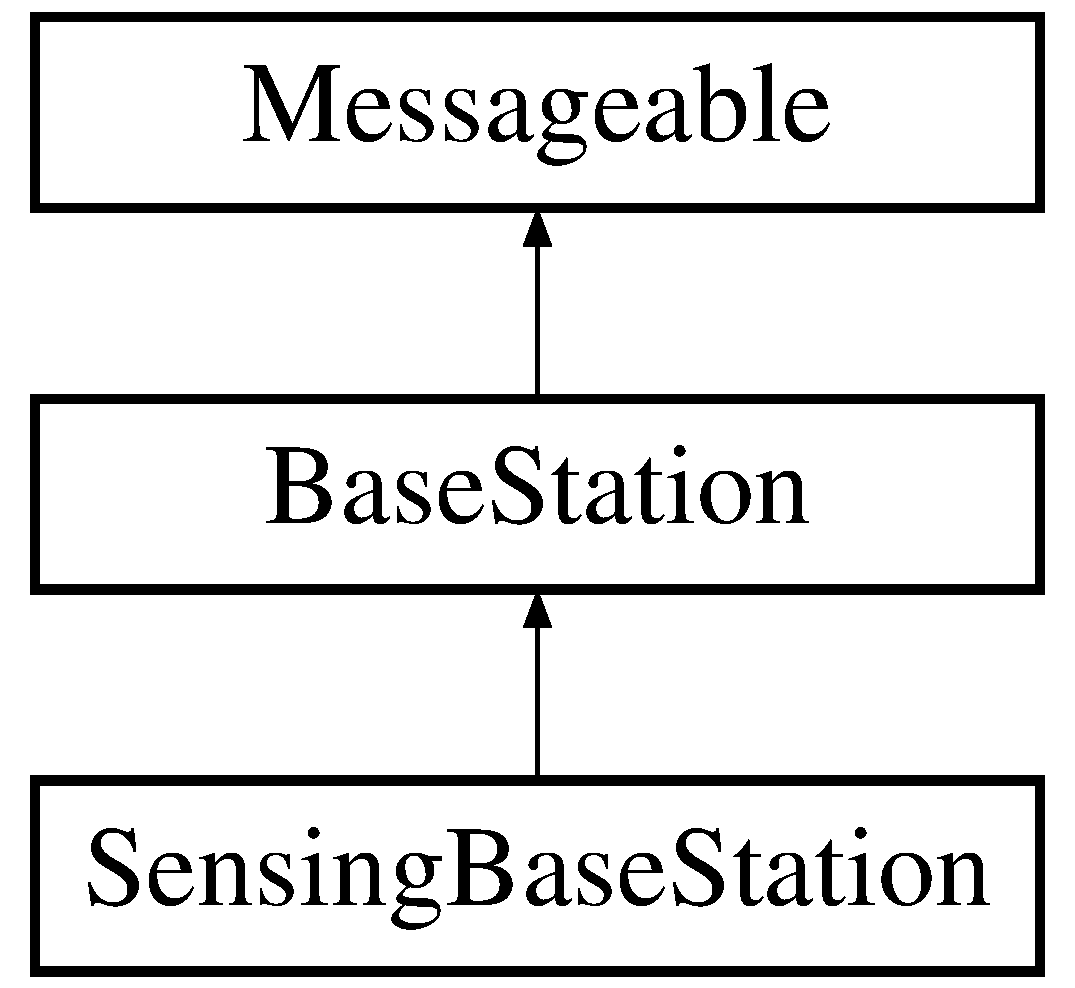
\includegraphics[height=3.000000cm]{class_base_station}
\end{center}
\end{figure}
\subsection*{Public Member Functions}
\begin{DoxyCompactItemize}
\item 
{\bfseries Base\+Station} (\hyperlink{class_comm_mod}{Comm\+Mod} $\ast$cm, double xp, double yp, double zp)\hypertarget{class_base_station_aa969be6d1673b8ad27229652ab608473}{}\label{class_base_station_aa969be6d1673b8ad27229652ab608473}

\end{DoxyCompactItemize}
\subsection*{Additional Inherited Members}


The documentation for this class was generated from the following files\+:\begin{DoxyCompactItemize}
\item 
/home/will/\+Documents/effacious-\/octo-\/weasel/code/simulator/Base\+Station.\+hpp\item 
/home/will/\+Documents/effacious-\/octo-\/weasel/code/simulator/Base\+Station.\+cpp\end{DoxyCompactItemize}

\hypertarget{class_comm_mod}{}\section{Comm\+Mod Class Reference}
\label{class_comm_mod}\index{Comm\+Mod@{Comm\+Mod}}


{\ttfamily \#include $<$Comm\+Mod.\+hpp$>$}

\subsection*{Public Member Functions}
\begin{DoxyCompactItemize}
\item 
\hyperlink{class_comm_mod_a00ab1077257c3672f8036468aecbf234}{Comm\+Mod} (\hyperlink{class_environment}{Environment} $\ast$env)
\item 
void \hyperlink{class_comm_mod_ab2e096b71516134bc0cb9bae4a965ef7}{set\+\_\+messageable} (\hyperlink{class_messageable}{Messageable} $\ast$msg)
\item 
void \hyperlink{class_comm_mod_abcfe15ea4ed5b27d77d2613cc4e786a3}{broadcast} (std\+::string message, double x\+Pos, double y\+Pos, double z\+Pos, double range)
\item 
void \hyperlink{class_comm_mod_af3e34b66c07a5c1e35a806443d0bca8c}{broadcast} (\hyperlink{class_message}{Message} $\ast$message, double x\+Pos, double y\+Pos, double z\+Pos, double range)
\item 
void \hyperlink{class_comm_mod_a696711acc752f9c2c60865194de3287f}{push\+\_\+out\+\_\+message} (\hyperlink{class_message}{Message} $\ast$message)
\item 
void \hyperlink{class_comm_mod_a2acc6cb30eb7c9d55e3893da147db839}{push\+\_\+in\+\_\+message} (std\+::string message)
\item 
virtual void \hyperlink{class_comm_mod_a48b1d970ce600043bf2b610ae113e825}{comm\+\_\+function} ()=0
\item 
double \hyperlink{class_comm_mod_a7415ee1b2835f8cb0d650df6ed80622a}{get\+Time} ()
\end{DoxyCompactItemize}
\subsection*{Protected Attributes}
\begin{DoxyCompactItemize}
\item 
std\+::queue$<$ \hyperlink{class_message}{Message} $\ast$ $>$ \hyperlink{class_comm_mod_abbd4cbdbb8c4b8680a20aea400e2eabc}{out\+Queue}
\item 
std\+::queue$<$ std\+::string $>$ \hyperlink{class_comm_mod_a4d31d6d1741edaaf0ec840ff8bb30047}{in\+Queue}
\item 
\hyperlink{class_environment}{Environment} $\ast$ \hyperlink{class_comm_mod_ae4953d3dd38bca7f71c309964636af91}{environment}
\item 
\hyperlink{class_messageable}{Messageable} $\ast$ \hyperlink{class_comm_mod_ae45eb57f9d550eb7c0dbb9311a71f72e}{messageable}
\end{DoxyCompactItemize}


\subsection{Constructor \& Destructor Documentation}
\index{Comm\+Mod@{Comm\+Mod}!Comm\+Mod@{Comm\+Mod}}
\index{Comm\+Mod@{Comm\+Mod}!Comm\+Mod@{Comm\+Mod}}
\subsubsection[{\texorpdfstring{Comm\+Mod(\+Environment $\ast$env)}{CommMod(Environment *env)}}]{\setlength{\rightskip}{0pt plus 5cm}Comm\+Mod\+::\+Comm\+Mod (
\begin{DoxyParamCaption}
\item[{{\bf Environment} $\ast$}]{env}
\end{DoxyParamCaption}
)}\hypertarget{class_comm_mod_a00ab1077257c3672f8036468aecbf234}{}\label{class_comm_mod_a00ab1077257c3672f8036468aecbf234}


\subsection{Member Function Documentation}
\index{Comm\+Mod@{Comm\+Mod}!broadcast@{broadcast}}
\index{broadcast@{broadcast}!Comm\+Mod@{Comm\+Mod}}
\subsubsection[{\texorpdfstring{broadcast(std\+::string message, double x\+Pos, double y\+Pos, double z\+Pos, double range)}{broadcast(std::string message, double xPos, double yPos, double zPos, double range)}}]{\setlength{\rightskip}{0pt plus 5cm}void Comm\+Mod\+::broadcast (
\begin{DoxyParamCaption}
\item[{std\+::string}]{message, }
\item[{double}]{x\+Pos, }
\item[{double}]{y\+Pos, }
\item[{double}]{z\+Pos, }
\item[{double}]{range}
\end{DoxyParamCaption}
)}\hypertarget{class_comm_mod_abcfe15ea4ed5b27d77d2613cc4e786a3}{}\label{class_comm_mod_abcfe15ea4ed5b27d77d2613cc4e786a3}
\index{Comm\+Mod@{Comm\+Mod}!broadcast@{broadcast}}
\index{broadcast@{broadcast}!Comm\+Mod@{Comm\+Mod}}
\subsubsection[{\texorpdfstring{broadcast(\+Message $\ast$message, double x\+Pos, double y\+Pos, double z\+Pos, double range)}{broadcast(Message *message, double xPos, double yPos, double zPos, double range)}}]{\setlength{\rightskip}{0pt plus 5cm}void Comm\+Mod\+::broadcast (
\begin{DoxyParamCaption}
\item[{{\bf Message} $\ast$}]{message, }
\item[{double}]{x\+Pos, }
\item[{double}]{y\+Pos, }
\item[{double}]{z\+Pos, }
\item[{double}]{range}
\end{DoxyParamCaption}
)}\hypertarget{class_comm_mod_af3e34b66c07a5c1e35a806443d0bca8c}{}\label{class_comm_mod_af3e34b66c07a5c1e35a806443d0bca8c}
\index{Comm\+Mod@{Comm\+Mod}!comm\+\_\+function@{comm\+\_\+function}}
\index{comm\+\_\+function@{comm\+\_\+function}!Comm\+Mod@{Comm\+Mod}}
\subsubsection[{\texorpdfstring{comm\+\_\+function()=0}{comm_function()=0}}]{\setlength{\rightskip}{0pt plus 5cm}virtual void Comm\+Mod\+::comm\+\_\+function (
\begin{DoxyParamCaption}
{}
\end{DoxyParamCaption}
)\hspace{0.3cm}{\ttfamily [pure virtual]}}\hypertarget{class_comm_mod_a48b1d970ce600043bf2b610ae113e825}{}\label{class_comm_mod_a48b1d970ce600043bf2b610ae113e825}
\index{Comm\+Mod@{Comm\+Mod}!get\+Time@{get\+Time}}
\index{get\+Time@{get\+Time}!Comm\+Mod@{Comm\+Mod}}
\subsubsection[{\texorpdfstring{get\+Time()}{getTime()}}]{\setlength{\rightskip}{0pt plus 5cm}double Comm\+Mod\+::get\+Time (
\begin{DoxyParamCaption}
{}
\end{DoxyParamCaption}
)}\hypertarget{class_comm_mod_a7415ee1b2835f8cb0d650df6ed80622a}{}\label{class_comm_mod_a7415ee1b2835f8cb0d650df6ed80622a}
\index{Comm\+Mod@{Comm\+Mod}!push\+\_\+in\+\_\+message@{push\+\_\+in\+\_\+message}}
\index{push\+\_\+in\+\_\+message@{push\+\_\+in\+\_\+message}!Comm\+Mod@{Comm\+Mod}}
\subsubsection[{\texorpdfstring{push\+\_\+in\+\_\+message(std\+::string message)}{push_in_message(std::string message)}}]{\setlength{\rightskip}{0pt plus 5cm}void Comm\+Mod\+::push\+\_\+in\+\_\+message (
\begin{DoxyParamCaption}
\item[{std\+::string}]{message}
\end{DoxyParamCaption}
)}\hypertarget{class_comm_mod_a2acc6cb30eb7c9d55e3893da147db839}{}\label{class_comm_mod_a2acc6cb30eb7c9d55e3893da147db839}
\index{Comm\+Mod@{Comm\+Mod}!push\+\_\+out\+\_\+message@{push\+\_\+out\+\_\+message}}
\index{push\+\_\+out\+\_\+message@{push\+\_\+out\+\_\+message}!Comm\+Mod@{Comm\+Mod}}
\subsubsection[{\texorpdfstring{push\+\_\+out\+\_\+message(\+Message $\ast$message)}{push_out_message(Message *message)}}]{\setlength{\rightskip}{0pt plus 5cm}void Comm\+Mod\+::push\+\_\+out\+\_\+message (
\begin{DoxyParamCaption}
\item[{{\bf Message} $\ast$}]{message}
\end{DoxyParamCaption}
)}\hypertarget{class_comm_mod_a696711acc752f9c2c60865194de3287f}{}\label{class_comm_mod_a696711acc752f9c2c60865194de3287f}
\index{Comm\+Mod@{Comm\+Mod}!set\+\_\+messageable@{set\+\_\+messageable}}
\index{set\+\_\+messageable@{set\+\_\+messageable}!Comm\+Mod@{Comm\+Mod}}
\subsubsection[{\texorpdfstring{set\+\_\+messageable(\+Messageable $\ast$msg)}{set_messageable(Messageable *msg)}}]{\setlength{\rightskip}{0pt plus 5cm}void Comm\+Mod\+::set\+\_\+messageable (
\begin{DoxyParamCaption}
\item[{{\bf Messageable} $\ast$}]{msg}
\end{DoxyParamCaption}
)}\hypertarget{class_comm_mod_ab2e096b71516134bc0cb9bae4a965ef7}{}\label{class_comm_mod_ab2e096b71516134bc0cb9bae4a965ef7}


\subsection{Member Data Documentation}
\index{Comm\+Mod@{Comm\+Mod}!environment@{environment}}
\index{environment@{environment}!Comm\+Mod@{Comm\+Mod}}
\subsubsection[{\texorpdfstring{environment}{environment}}]{\setlength{\rightskip}{0pt plus 5cm}{\bf Environment}$\ast$ Comm\+Mod\+::environment\hspace{0.3cm}{\ttfamily [protected]}}\hypertarget{class_comm_mod_ae4953d3dd38bca7f71c309964636af91}{}\label{class_comm_mod_ae4953d3dd38bca7f71c309964636af91}
\index{Comm\+Mod@{Comm\+Mod}!in\+Queue@{in\+Queue}}
\index{in\+Queue@{in\+Queue}!Comm\+Mod@{Comm\+Mod}}
\subsubsection[{\texorpdfstring{in\+Queue}{inQueue}}]{\setlength{\rightskip}{0pt plus 5cm}std\+::queue$<$std\+::string$>$ Comm\+Mod\+::in\+Queue\hspace{0.3cm}{\ttfamily [protected]}}\hypertarget{class_comm_mod_a4d31d6d1741edaaf0ec840ff8bb30047}{}\label{class_comm_mod_a4d31d6d1741edaaf0ec840ff8bb30047}
\index{Comm\+Mod@{Comm\+Mod}!messageable@{messageable}}
\index{messageable@{messageable}!Comm\+Mod@{Comm\+Mod}}
\subsubsection[{\texorpdfstring{messageable}{messageable}}]{\setlength{\rightskip}{0pt plus 5cm}{\bf Messageable}$\ast$ Comm\+Mod\+::messageable\hspace{0.3cm}{\ttfamily [protected]}}\hypertarget{class_comm_mod_ae45eb57f9d550eb7c0dbb9311a71f72e}{}\label{class_comm_mod_ae45eb57f9d550eb7c0dbb9311a71f72e}
\index{Comm\+Mod@{Comm\+Mod}!out\+Queue@{out\+Queue}}
\index{out\+Queue@{out\+Queue}!Comm\+Mod@{Comm\+Mod}}
\subsubsection[{\texorpdfstring{out\+Queue}{outQueue}}]{\setlength{\rightskip}{0pt plus 5cm}std\+::queue$<${\bf Message}$\ast$$>$ Comm\+Mod\+::out\+Queue\hspace{0.3cm}{\ttfamily [protected]}}\hypertarget{class_comm_mod_abbd4cbdbb8c4b8680a20aea400e2eabc}{}\label{class_comm_mod_abbd4cbdbb8c4b8680a20aea400e2eabc}


The documentation for this class was generated from the following files\+:\begin{DoxyCompactItemize}
\item 
D\+:/\+My Documents/\+University Year 4/\+C\+S410 Group Project/effacious-\/octo-\/weasel/code/simulator/\hyperlink{_comm_mod_8hpp}{Comm\+Mod.\+hpp}\item 
D\+:/\+My Documents/\+University Year 4/\+C\+S410 Group Project/effacious-\/octo-\/weasel/code/simulator/\hyperlink{_comm_mod_8cpp}{Comm\+Mod.\+cpp}\end{DoxyCompactItemize}

\hypertarget{struct_coord}{}\section{Coord Struct Reference}
\label{struct_coord}\index{Coord@{Coord}}


{\ttfamily \#include $<$Messageable.\+hpp$>$}

\subsection*{Public Attributes}
\begin{DoxyCompactItemize}
\item 
double \hyperlink{struct_coord_a0172a22ee75843a96e3a84ebc25f3de7}{x}
\item 
double \hyperlink{struct_coord_af6e543e0522076e717bae53102655b87}{y}
\item 
double \hyperlink{struct_coord_a2bf056108a79437171f18490afbdce2d}{z}
\end{DoxyCompactItemize}


\subsection{Member Data Documentation}
\index{Coord@{Coord}!x@{x}}
\index{x@{x}!Coord@{Coord}}
\subsubsection[{\texorpdfstring{x}{x}}]{\setlength{\rightskip}{0pt plus 5cm}double Coord\+::x}\hypertarget{struct_coord_a0172a22ee75843a96e3a84ebc25f3de7}{}\label{struct_coord_a0172a22ee75843a96e3a84ebc25f3de7}
\index{Coord@{Coord}!y@{y}}
\index{y@{y}!Coord@{Coord}}
\subsubsection[{\texorpdfstring{y}{y}}]{\setlength{\rightskip}{0pt plus 5cm}double Coord\+::y}\hypertarget{struct_coord_af6e543e0522076e717bae53102655b87}{}\label{struct_coord_af6e543e0522076e717bae53102655b87}
\index{Coord@{Coord}!z@{z}}
\index{z@{z}!Coord@{Coord}}
\subsubsection[{\texorpdfstring{z}{z}}]{\setlength{\rightskip}{0pt plus 5cm}double Coord\+::z}\hypertarget{struct_coord_a2bf056108a79437171f18490afbdce2d}{}\label{struct_coord_a2bf056108a79437171f18490afbdce2d}


The documentation for this struct was generated from the following file\+:\begin{DoxyCompactItemize}
\item 
/home/will/\+Documents/effacious-\/octo-\/weasel/code/simulator/\hyperlink{_messageable_8hpp}{Messageable.\+hpp}\end{DoxyCompactItemize}

\hypertarget{class_drone}{}\section{Drone Class Reference}
\label{class_drone}\index{Drone@{Drone}}


{\ttfamily \#include $<$Drone.\+hpp$>$}

Inheritance diagram for Drone\+:\begin{figure}[H]
\begin{center}
\leavevmode
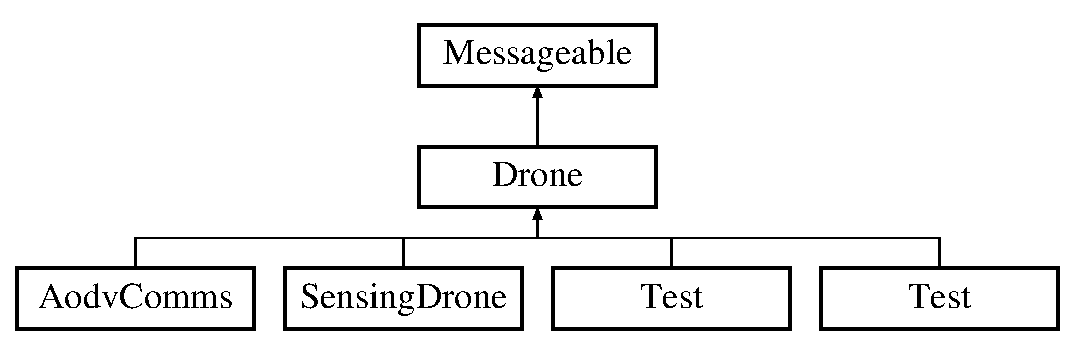
\includegraphics[height=2.000000cm]{class_drone}
\end{center}
\end{figure}
\subsection*{Public Member Functions}
\begin{DoxyCompactItemize}
\item 
\hyperlink{class_drone_a671923cbf775d479aa11f469b82503f3}{Drone} (\hyperlink{class_comm_mod}{Comm\+Mod} $\ast$cm, double iX, double iY, double iZ, double \hyperlink{class_drone_a9dcad921c51f4e7455ef79c16261404c}{max\+Speed}, \hyperlink{class_environment}{Environment} $\ast$e)
\item 
bool \hyperlink{class_drone_a5181059ce456e7ccdf3366ee1f8156db}{is\+Alive} ()
\item 
void \hyperlink{class_drone_a4a53691055a0561e5069ea1482ac893b}{upkeep} ()
\end{DoxyCompactItemize}
\subsection*{Protected Member Functions}
\begin{DoxyCompactItemize}
\item 
void \hyperlink{class_drone_a87b644ed6c297252a0930b4a915a553e}{kill} ()
\item 
void \hyperlink{class_drone_a81c5a726112abba3d686e95baccd54be}{turn} (double d\+Angle)
\item 
void \hyperlink{class_drone_ae7ebc3df04a42e9c49389ab2868d102d}{move} (\hyperlink{_drone_8hpp_a224b9163917ac32fc95a60d8c1eec3aa}{Direction} direction, double speed, double distance)
\item 
double \hyperlink{class_drone_a780e43c6486a26eb47a37295ea510269}{get\+Max\+Speed} ()
\item 
double \hyperlink{class_drone_abd485e52d2ac2d6d81038665495bb480}{sense} (std\+::string type)
\end{DoxyCompactItemize}
\subsection*{Private Attributes}
\begin{DoxyCompactItemize}
\item 
double \hyperlink{class_drone_a58d0d1070b3339121051cb88c8edc5bf}{o\+Time}
\item 
bool \hyperlink{class_drone_aea356a33311281ec16bba90066af5142}{alive} = true
\item 
\hyperlink{_drone_8hpp_a224b9163917ac32fc95a60d8c1eec3aa}{Direction} \hyperlink{class_drone_a9489e36ee8f7c1c4f9ea1374fa2deed8}{dir}
\item 
double \hyperlink{class_drone_a9dcad921c51f4e7455ef79c16261404c}{max\+Speed}
\item 
double \hyperlink{class_drone_a88b4a0066796c01715b4313bf13f1468}{ang} = 0
\item 
\hyperlink{class_environment}{Environment} $\ast$ \hyperlink{class_drone_a283a1a6532801f59250478d20fa5392f}{env}
\item 
double \hyperlink{class_drone_a1320892a8f0d71d63a36e23079f7d56c}{move\+DR}
\item 
double \hyperlink{class_drone_a97270a4291d82a57331669171bd80bc1}{move\+Spd}
\end{DoxyCompactItemize}
\subsection*{Additional Inherited Members}


\subsection{Constructor \& Destructor Documentation}
\index{Drone@{Drone}!Drone@{Drone}}
\index{Drone@{Drone}!Drone@{Drone}}
\subsubsection[{\texorpdfstring{Drone(\+Comm\+Mod $\ast$cm, double i\+X, double i\+Y, double i\+Z, double max\+Speed, Environment $\ast$e)}{Drone(CommMod *cm, double iX, double iY, double iZ, double maxSpeed, Environment *e)}}]{\setlength{\rightskip}{0pt plus 5cm}Drone\+::\+Drone (
\begin{DoxyParamCaption}
\item[{{\bf Comm\+Mod} $\ast$}]{cm, }
\item[{double}]{iX, }
\item[{double}]{iY, }
\item[{double}]{iZ, }
\item[{double}]{max\+Speed, }
\item[{{\bf Environment} $\ast$}]{e}
\end{DoxyParamCaption}
)}\hypertarget{class_drone_a671923cbf775d479aa11f469b82503f3}{}\label{class_drone_a671923cbf775d479aa11f469b82503f3}


\subsection{Member Function Documentation}
\index{Drone@{Drone}!get\+Max\+Speed@{get\+Max\+Speed}}
\index{get\+Max\+Speed@{get\+Max\+Speed}!Drone@{Drone}}
\subsubsection[{\texorpdfstring{get\+Max\+Speed()}{getMaxSpeed()}}]{\setlength{\rightskip}{0pt plus 5cm}double Drone\+::get\+Max\+Speed (
\begin{DoxyParamCaption}
{}
\end{DoxyParamCaption}
)\hspace{0.3cm}{\ttfamily [protected]}}\hypertarget{class_drone_a780e43c6486a26eb47a37295ea510269}{}\label{class_drone_a780e43c6486a26eb47a37295ea510269}
\index{Drone@{Drone}!is\+Alive@{is\+Alive}}
\index{is\+Alive@{is\+Alive}!Drone@{Drone}}
\subsubsection[{\texorpdfstring{is\+Alive()}{isAlive()}}]{\setlength{\rightskip}{0pt plus 5cm}bool Drone\+::is\+Alive (
\begin{DoxyParamCaption}
{}
\end{DoxyParamCaption}
)}\hypertarget{class_drone_a5181059ce456e7ccdf3366ee1f8156db}{}\label{class_drone_a5181059ce456e7ccdf3366ee1f8156db}
\index{Drone@{Drone}!kill@{kill}}
\index{kill@{kill}!Drone@{Drone}}
\subsubsection[{\texorpdfstring{kill()}{kill()}}]{\setlength{\rightskip}{0pt plus 5cm}void Drone\+::kill (
\begin{DoxyParamCaption}
{}
\end{DoxyParamCaption}
)\hspace{0.3cm}{\ttfamily [protected]}}\hypertarget{class_drone_a87b644ed6c297252a0930b4a915a553e}{}\label{class_drone_a87b644ed6c297252a0930b4a915a553e}
\index{Drone@{Drone}!move@{move}}
\index{move@{move}!Drone@{Drone}}
\subsubsection[{\texorpdfstring{move(\+Direction direction, double speed, double distance)}{move(Direction direction, double speed, double distance)}}]{\setlength{\rightskip}{0pt plus 5cm}void Drone\+::move (
\begin{DoxyParamCaption}
\item[{{\bf Direction}}]{direction, }
\item[{double}]{speed, }
\item[{double}]{distance}
\end{DoxyParamCaption}
)\hspace{0.3cm}{\ttfamily [protected]}}\hypertarget{class_drone_ae7ebc3df04a42e9c49389ab2868d102d}{}\label{class_drone_ae7ebc3df04a42e9c49389ab2868d102d}
\index{Drone@{Drone}!sense@{sense}}
\index{sense@{sense}!Drone@{Drone}}
\subsubsection[{\texorpdfstring{sense(std\+::string type)}{sense(std::string type)}}]{\setlength{\rightskip}{0pt plus 5cm}double Drone\+::sense (
\begin{DoxyParamCaption}
\item[{std\+::string}]{type}
\end{DoxyParamCaption}
)\hspace{0.3cm}{\ttfamily [protected]}}\hypertarget{class_drone_abd485e52d2ac2d6d81038665495bb480}{}\label{class_drone_abd485e52d2ac2d6d81038665495bb480}
\index{Drone@{Drone}!turn@{turn}}
\index{turn@{turn}!Drone@{Drone}}
\subsubsection[{\texorpdfstring{turn(double d\+Angle)}{turn(double dAngle)}}]{\setlength{\rightskip}{0pt plus 5cm}void Drone\+::turn (
\begin{DoxyParamCaption}
\item[{double}]{d\+Angle}
\end{DoxyParamCaption}
)\hspace{0.3cm}{\ttfamily [protected]}}\hypertarget{class_drone_a81c5a726112abba3d686e95baccd54be}{}\label{class_drone_a81c5a726112abba3d686e95baccd54be}
\index{Drone@{Drone}!upkeep@{upkeep}}
\index{upkeep@{upkeep}!Drone@{Drone}}
\subsubsection[{\texorpdfstring{upkeep()}{upkeep()}}]{\setlength{\rightskip}{0pt plus 5cm}void Drone\+::upkeep (
\begin{DoxyParamCaption}
{}
\end{DoxyParamCaption}
)}\hypertarget{class_drone_a4a53691055a0561e5069ea1482ac893b}{}\label{class_drone_a4a53691055a0561e5069ea1482ac893b}


\subsection{Member Data Documentation}
\index{Drone@{Drone}!alive@{alive}}
\index{alive@{alive}!Drone@{Drone}}
\subsubsection[{\texorpdfstring{alive}{alive}}]{\setlength{\rightskip}{0pt plus 5cm}bool Drone\+::alive = true\hspace{0.3cm}{\ttfamily [private]}}\hypertarget{class_drone_aea356a33311281ec16bba90066af5142}{}\label{class_drone_aea356a33311281ec16bba90066af5142}
\index{Drone@{Drone}!ang@{ang}}
\index{ang@{ang}!Drone@{Drone}}
\subsubsection[{\texorpdfstring{ang}{ang}}]{\setlength{\rightskip}{0pt plus 5cm}double Drone\+::ang = 0\hspace{0.3cm}{\ttfamily [private]}}\hypertarget{class_drone_a88b4a0066796c01715b4313bf13f1468}{}\label{class_drone_a88b4a0066796c01715b4313bf13f1468}
\index{Drone@{Drone}!dir@{dir}}
\index{dir@{dir}!Drone@{Drone}}
\subsubsection[{\texorpdfstring{dir}{dir}}]{\setlength{\rightskip}{0pt plus 5cm}{\bf Direction} Drone\+::dir\hspace{0.3cm}{\ttfamily [private]}}\hypertarget{class_drone_a9489e36ee8f7c1c4f9ea1374fa2deed8}{}\label{class_drone_a9489e36ee8f7c1c4f9ea1374fa2deed8}
\index{Drone@{Drone}!env@{env}}
\index{env@{env}!Drone@{Drone}}
\subsubsection[{\texorpdfstring{env}{env}}]{\setlength{\rightskip}{0pt plus 5cm}{\bf Environment}$\ast$ Drone\+::env\hspace{0.3cm}{\ttfamily [private]}}\hypertarget{class_drone_a283a1a6532801f59250478d20fa5392f}{}\label{class_drone_a283a1a6532801f59250478d20fa5392f}
\index{Drone@{Drone}!max\+Speed@{max\+Speed}}
\index{max\+Speed@{max\+Speed}!Drone@{Drone}}
\subsubsection[{\texorpdfstring{max\+Speed}{maxSpeed}}]{\setlength{\rightskip}{0pt plus 5cm}double Drone\+::max\+Speed\hspace{0.3cm}{\ttfamily [private]}}\hypertarget{class_drone_a9dcad921c51f4e7455ef79c16261404c}{}\label{class_drone_a9dcad921c51f4e7455ef79c16261404c}
\index{Drone@{Drone}!move\+DR@{move\+DR}}
\index{move\+DR@{move\+DR}!Drone@{Drone}}
\subsubsection[{\texorpdfstring{move\+DR}{moveDR}}]{\setlength{\rightskip}{0pt plus 5cm}double Drone\+::move\+DR\hspace{0.3cm}{\ttfamily [private]}}\hypertarget{class_drone_a1320892a8f0d71d63a36e23079f7d56c}{}\label{class_drone_a1320892a8f0d71d63a36e23079f7d56c}
\index{Drone@{Drone}!move\+Spd@{move\+Spd}}
\index{move\+Spd@{move\+Spd}!Drone@{Drone}}
\subsubsection[{\texorpdfstring{move\+Spd}{moveSpd}}]{\setlength{\rightskip}{0pt plus 5cm}double Drone\+::move\+Spd\hspace{0.3cm}{\ttfamily [private]}}\hypertarget{class_drone_a97270a4291d82a57331669171bd80bc1}{}\label{class_drone_a97270a4291d82a57331669171bd80bc1}
\index{Drone@{Drone}!o\+Time@{o\+Time}}
\index{o\+Time@{o\+Time}!Drone@{Drone}}
\subsubsection[{\texorpdfstring{o\+Time}{oTime}}]{\setlength{\rightskip}{0pt plus 5cm}double Drone\+::o\+Time\hspace{0.3cm}{\ttfamily [private]}}\hypertarget{class_drone_a58d0d1070b3339121051cb88c8edc5bf}{}\label{class_drone_a58d0d1070b3339121051cb88c8edc5bf}


The documentation for this class was generated from the following files\+:\begin{DoxyCompactItemize}
\item 
D\+:/\+My Documents/\+University Year 4/\+C\+S410 Group Project/effacious-\/octo-\/weasel/code/simulator/\hyperlink{_drone_8hpp}{Drone.\+hpp}\item 
D\+:/\+My Documents/\+University Year 4/\+C\+S410 Group Project/effacious-\/octo-\/weasel/code/simulator/\hyperlink{_drone_8cpp}{Drone.\+cpp}\end{DoxyCompactItemize}

\hypertarget{class_environment}{}\section{Environment Class Reference}
\label{class_environment}\index{Environment@{Environment}}
\subsection*{Public Member Functions}
\begin{DoxyCompactItemize}
\item 
{\bfseries Environment} (std\+::map$<$ std\+::string, data\+\_\+type $>$, std\+::function$<$ std\+::string(std\+::string)$>$, double timestep)\hypertarget{class_environment_aaddf445dbf4217a68a373e183a2bfb0c}{}\label{class_environment_aaddf445dbf4217a68a373e183a2bfb0c}

\item 
{\bfseries Environment} (std\+::map$<$ std\+::string, data\+\_\+type $>$, double timestep)\hypertarget{class_environment_a098fcd6da9a033833095ec76f60aab0d}{}\label{class_environment_a098fcd6da9a033833095ec76f60aab0d}

\item 
void {\bfseries broadcast} (std\+::string message, double x\+Origin, double y\+Origin, double z\+Origin, double range, \hyperlink{class_comm_mod}{Comm\+Mod} $\ast$)\hypertarget{class_environment_a8d5bb36197739b8fb8532755210865c4}{}\label{class_environment_a8d5bb36197739b8fb8532755210865c4}

\item 
void {\bfseries add\+Data} (std\+::string type, data\+\_\+type d)\hypertarget{class_environment_abadae98bdccb015d49c6f94c97a8bf82}{}\label{class_environment_abadae98bdccb015d49c6f94c97a8bf82}

\item 
void {\bfseries add\+Drone} (\hyperlink{class_drone}{Drone} $\ast$m)\hypertarget{class_environment_a95654e6bc17cbd781453fdb256fa979b}{}\label{class_environment_a95654e6bc17cbd781453fdb256fa979b}

\item 
void {\bfseries set\+Base\+Station} (\hyperlink{class_base_station}{Base\+Station} $\ast$m)\hypertarget{class_environment_aa06fdaa6619d957c10d858c176f3f307}{}\label{class_environment_aa06fdaa6619d957c10d858c176f3f307}

\item 
double {\bfseries get\+Data} (std\+::string type, double x, double y, double z)\hypertarget{class_environment_a0a2b32ecbd52779d17b3d9a483aa6d24}{}\label{class_environment_a0a2b32ecbd52779d17b3d9a483aa6d24}

\item 
double {\bfseries get\+Time} ()\hypertarget{class_environment_a03d9d2db949b5491e60e922d9a33769b}{}\label{class_environment_a03d9d2db949b5491e60e922d9a33769b}

\item 
void {\bfseries run} ()\hypertarget{class_environment_a41a43b88702fff5df95e98d10e49f541}{}\label{class_environment_a41a43b88702fff5df95e98d10e49f541}

\end{DoxyCompactItemize}
\subsection*{Private Types}
\begin{DoxyCompactItemize}
\item 
typedef std\+::vector$<$ std\+::vector$<$ std\+::vector$<$ double $>$ $>$ $>$ {\bfseries data\+\_\+type}\hypertarget{class_environment_a7ac989afdd3bde4ea860c985ed1f8479}{}\label{class_environment_a7ac989afdd3bde4ea860c985ed1f8479}

\end{DoxyCompactItemize}
\subsection*{Private Attributes}
\begin{DoxyCompactItemize}
\item 
double {\bfseries time\+Elapsed}\hypertarget{class_environment_a94758a1936023963eafaa129bb84f89d}{}\label{class_environment_a94758a1936023963eafaa129bb84f89d}

\item 
double {\bfseries time\+Step}\hypertarget{class_environment_a0eac119e9f0130f836f04224612dfb16}{}\label{class_environment_a0eac119e9f0130f836f04224612dfb16}

\item 
\hyperlink{class_base_station}{Base\+Station} $\ast$ {\bfseries base\+Station}\hypertarget{class_environment_a01e059baab4daf8833a638fab15eab31}{}\label{class_environment_a01e059baab4daf8833a638fab15eab31}

\item 
std\+::vector$<$ \hyperlink{class_drone}{Drone} $\ast$ $>$ {\bfseries drones}\hypertarget{class_environment_a3119b68685b61fc60e0a76918fa83f0a}{}\label{class_environment_a3119b68685b61fc60e0a76918fa83f0a}

\item 
std\+::map$<$ std\+::string, data\+\_\+type $>$ {\bfseries data}\hypertarget{class_environment_a8f4846d547c4891a4a2493157c8f76d6}{}\label{class_environment_a8f4846d547c4891a4a2493157c8f76d6}

\item 
std\+::function$<$ std\+::string(std\+::string)$>$ {\bfseries noise\+Fun}\hypertarget{class_environment_a95650888a9bfb308a650c049a95cb6cb}{}\label{class_environment_a95650888a9bfb308a650c049a95cb6cb}

\end{DoxyCompactItemize}


The documentation for this class was generated from the following files\+:\begin{DoxyCompactItemize}
\item 
/home/will/\+Documents/effacious-\/octo-\/weasel/code/simulator/Environment.\+hpp\item 
/home/will/\+Documents/effacious-\/octo-\/weasel/code/simulator/Environment.\+cpp\end{DoxyCompactItemize}

\hypertarget{class_message}{}\section{Message Class Reference}
\label{class_message}\index{Message@{Message}}


{\ttfamily \#include $<$Message.\+hpp$>$}

\subsection*{Public Member Functions}
\begin{DoxyCompactItemize}
\item 
\hyperlink{class_message_aa222cbc5bf7865d5464a841740f45c11}{Message} (std\+::string \hyperlink{class_message_ae9dead264183a4243c120026e6259b6f}{type})
\item 
time\+\_\+t \hyperlink{class_message_a5c9fecc6bf5fa404a04b89d7585a757c}{get\+\_\+current\+\_\+time} ()
\item 
virtual std\+::string \hyperlink{class_message_af65196e1bf4dfa1e44f59757612d3586}{to\+\_\+string} ()=0
\item 
std\+::string \hyperlink{class_message_ae3680358818bc391a3fb25bfc6fc57d6}{get\+\_\+type} ()
\end{DoxyCompactItemize}
\subsection*{Private Attributes}
\begin{DoxyCompactItemize}
\item 
std\+::string \hyperlink{class_message_ae9dead264183a4243c120026e6259b6f}{type}
\end{DoxyCompactItemize}


\subsection{Constructor \& Destructor Documentation}
\index{Message@{Message}!Message@{Message}}
\index{Message@{Message}!Message@{Message}}
\subsubsection[{\texorpdfstring{Message(std\+::string type)}{Message(std::string type)}}]{\setlength{\rightskip}{0pt plus 5cm}Message\+::\+Message (
\begin{DoxyParamCaption}
\item[{std\+::string}]{type}
\end{DoxyParamCaption}
)}\hypertarget{class_message_aa222cbc5bf7865d5464a841740f45c11}{}\label{class_message_aa222cbc5bf7865d5464a841740f45c11}


\subsection{Member Function Documentation}
\index{Message@{Message}!get\+\_\+current\+\_\+time@{get\+\_\+current\+\_\+time}}
\index{get\+\_\+current\+\_\+time@{get\+\_\+current\+\_\+time}!Message@{Message}}
\subsubsection[{\texorpdfstring{get\+\_\+current\+\_\+time()}{get_current_time()}}]{\setlength{\rightskip}{0pt plus 5cm}time\+\_\+t Message\+::get\+\_\+current\+\_\+time (
\begin{DoxyParamCaption}
{}
\end{DoxyParamCaption}
)}\hypertarget{class_message_a5c9fecc6bf5fa404a04b89d7585a757c}{}\label{class_message_a5c9fecc6bf5fa404a04b89d7585a757c}
\index{Message@{Message}!get\+\_\+type@{get\+\_\+type}}
\index{get\+\_\+type@{get\+\_\+type}!Message@{Message}}
\subsubsection[{\texorpdfstring{get\+\_\+type()}{get_type()}}]{\setlength{\rightskip}{0pt plus 5cm}std\+::string Message\+::get\+\_\+type (
\begin{DoxyParamCaption}
{}
\end{DoxyParamCaption}
)}\hypertarget{class_message_ae3680358818bc391a3fb25bfc6fc57d6}{}\label{class_message_ae3680358818bc391a3fb25bfc6fc57d6}
\index{Message@{Message}!to\+\_\+string@{to\+\_\+string}}
\index{to\+\_\+string@{to\+\_\+string}!Message@{Message}}
\subsubsection[{\texorpdfstring{to\+\_\+string()=0}{to_string()=0}}]{\setlength{\rightskip}{0pt plus 5cm}virtual std\+::string Message\+::to\+\_\+string (
\begin{DoxyParamCaption}
{}
\end{DoxyParamCaption}
)\hspace{0.3cm}{\ttfamily [pure virtual]}}\hypertarget{class_message_af65196e1bf4dfa1e44f59757612d3586}{}\label{class_message_af65196e1bf4dfa1e44f59757612d3586}


\subsection{Member Data Documentation}
\index{Message@{Message}!type@{type}}
\index{type@{type}!Message@{Message}}
\subsubsection[{\texorpdfstring{type}{type}}]{\setlength{\rightskip}{0pt plus 5cm}std\+::string Message\+::type\hspace{0.3cm}{\ttfamily [private]}}\hypertarget{class_message_ae9dead264183a4243c120026e6259b6f}{}\label{class_message_ae9dead264183a4243c120026e6259b6f}


The documentation for this class was generated from the following files\+:\begin{DoxyCompactItemize}
\item 
D\+:/\+My Documents/\+University Year 4/\+C\+S410 Group Project/effacious-\/octo-\/weasel/code/simulator/\hyperlink{_message_8hpp}{Message.\+hpp}\item 
D\+:/\+My Documents/\+University Year 4/\+C\+S410 Group Project/effacious-\/octo-\/weasel/code/simulator/\hyperlink{_message_8cpp}{Message.\+cpp}\end{DoxyCompactItemize}

\hypertarget{class_messageable}{}\section{Messageable Class Reference}
\label{class_messageable}\index{Messageable@{Messageable}}


{\ttfamily \#include $<$Messageable.\+hpp$>$}

Inheritance diagram for Messageable\+:\begin{figure}[H]
\begin{center}
\leavevmode
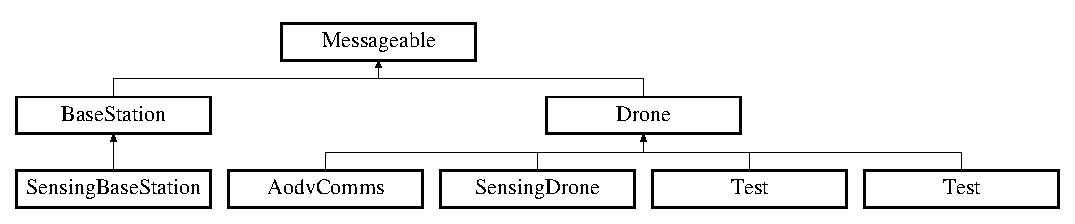
\includegraphics[height=2.000000cm]{class_messageable}
\end{center}
\end{figure}
\subsection*{Public Member Functions}
\begin{DoxyCompactItemize}
\item 
\hyperlink{class_messageable_a17da78cfa69fc760ece179365de9ef23}{Messageable} (\hyperlink{class_comm_mod}{Comm\+Mod} $\ast$cm, double xp, double yp, double zp)
\item 
void \hyperlink{class_messageable_aaadfd99f6f7a1ec8c8195232a48e3b15}{send\+\_\+message} (\hyperlink{class_message}{Message} $\ast$contents)
\item 
\hyperlink{class_message}{Message} $\ast$ \hyperlink{class_messageable_acca6e0ec0f301179e9bf5596b5b7d9a7}{wait\+\_\+for\+\_\+message} ()
\item 
void \hyperlink{class_messageable_a778d44d8365ed5927bf237d331593809}{push\+\_\+message} (\hyperlink{class_message}{Message} $\ast$contents)
\item 
void \hyperlink{class_messageable_a5e581d6cf3383931bb4749bbbe4d81ee}{receive\+\_\+message} (std\+::string contents)
\item 
\hyperlink{class_comm_mod}{Comm\+Mod} $\ast$ \hyperlink{class_messageable_a600102c71a3398e1ffe181c3e4e680a0}{get\+\_\+comm\+\_\+mod} ()
\item 
double \hyperlink{class_messageable_a95b2cc2dc0f0b5133cf490472b2b13bb}{getX} ()
\item 
double \hyperlink{class_messageable_a202416adb2413f9b5bc33c64ec2bc12e}{getY} ()
\item 
double \hyperlink{class_messageable_a7da3f0e2540087aa8933ec4cd99789ce}{getZ} ()
\item 
\hyperlink{struct_coord}{Coord} \hyperlink{class_messageable_a7f990ea00748e817ef7a20dd9ab8e88c}{get\+Position} ()
\item 
double \hyperlink{class_messageable_a695c9311c6ece88dd81ec325d24dc01e}{get\+Time} ()
\item 
virtual bool \hyperlink{class_messageable_adda0d24929a929b9d91c97da1fb91775}{message\+\_\+callback} (\hyperlink{class_message}{Message} $\ast$message)=0
\item 
virtual void \hyperlink{class_messageable_a82c2308b9fabe8e06664d17b3c018b75}{run} ()=0
\item 
void \hyperlink{class_messageable_ab39d542fbac3744a22161efbe0dc9ff7}{run\+Comm\+Mod} ()
\end{DoxyCompactItemize}
\subsection*{Protected Attributes}
\begin{DoxyCompactItemize}
\item 
std\+::queue$<$ \hyperlink{class_message}{Message} $\ast$ $>$ \hyperlink{class_messageable_a77bee602af65ca6708c3d77080298376}{in\+Queue}
\item 
\hyperlink{class_comm_mod}{Comm\+Mod} $\ast$ \hyperlink{class_messageable_a0c8ed985c63492656ab9e6d502c8f98e}{communications\+Module}
\item 
\hyperlink{struct_coord}{Coord} \hyperlink{class_messageable_a49ee36421becbc9f529f3d63d5e3169a}{position}
\end{DoxyCompactItemize}


\subsection{Constructor \& Destructor Documentation}
\index{Messageable@{Messageable}!Messageable@{Messageable}}
\index{Messageable@{Messageable}!Messageable@{Messageable}}
\subsubsection[{\texorpdfstring{Messageable(\+Comm\+Mod $\ast$cm, double xp, double yp, double zp)}{Messageable(CommMod *cm, double xp, double yp, double zp)}}]{\setlength{\rightskip}{0pt plus 5cm}Messageable\+::\+Messageable (
\begin{DoxyParamCaption}
\item[{{\bf Comm\+Mod} $\ast$}]{cm, }
\item[{double}]{xp, }
\item[{double}]{yp, }
\item[{double}]{zp}
\end{DoxyParamCaption}
)}\hypertarget{class_messageable_a17da78cfa69fc760ece179365de9ef23}{}\label{class_messageable_a17da78cfa69fc760ece179365de9ef23}


\subsection{Member Function Documentation}
\index{Messageable@{Messageable}!get\+\_\+comm\+\_\+mod@{get\+\_\+comm\+\_\+mod}}
\index{get\+\_\+comm\+\_\+mod@{get\+\_\+comm\+\_\+mod}!Messageable@{Messageable}}
\subsubsection[{\texorpdfstring{get\+\_\+comm\+\_\+mod()}{get_comm_mod()}}]{\setlength{\rightskip}{0pt plus 5cm}{\bf Comm\+Mod} $\ast$ Messageable\+::get\+\_\+comm\+\_\+mod (
\begin{DoxyParamCaption}
{}
\end{DoxyParamCaption}
)}\hypertarget{class_messageable_a600102c71a3398e1ffe181c3e4e680a0}{}\label{class_messageable_a600102c71a3398e1ffe181c3e4e680a0}
\index{Messageable@{Messageable}!get\+Position@{get\+Position}}
\index{get\+Position@{get\+Position}!Messageable@{Messageable}}
\subsubsection[{\texorpdfstring{get\+Position()}{getPosition()}}]{\setlength{\rightskip}{0pt plus 5cm}{\bf Coord} Messageable\+::get\+Position (
\begin{DoxyParamCaption}
{}
\end{DoxyParamCaption}
)}\hypertarget{class_messageable_a7f990ea00748e817ef7a20dd9ab8e88c}{}\label{class_messageable_a7f990ea00748e817ef7a20dd9ab8e88c}
\index{Messageable@{Messageable}!get\+Time@{get\+Time}}
\index{get\+Time@{get\+Time}!Messageable@{Messageable}}
\subsubsection[{\texorpdfstring{get\+Time()}{getTime()}}]{\setlength{\rightskip}{0pt plus 5cm}double Messageable\+::get\+Time (
\begin{DoxyParamCaption}
{}
\end{DoxyParamCaption}
)}\hypertarget{class_messageable_a695c9311c6ece88dd81ec325d24dc01e}{}\label{class_messageable_a695c9311c6ece88dd81ec325d24dc01e}
\index{Messageable@{Messageable}!getX@{getX}}
\index{getX@{getX}!Messageable@{Messageable}}
\subsubsection[{\texorpdfstring{get\+X()}{getX()}}]{\setlength{\rightskip}{0pt plus 5cm}double Messageable\+::getX (
\begin{DoxyParamCaption}
{}
\end{DoxyParamCaption}
)}\hypertarget{class_messageable_a95b2cc2dc0f0b5133cf490472b2b13bb}{}\label{class_messageable_a95b2cc2dc0f0b5133cf490472b2b13bb}
\index{Messageable@{Messageable}!getY@{getY}}
\index{getY@{getY}!Messageable@{Messageable}}
\subsubsection[{\texorpdfstring{get\+Y()}{getY()}}]{\setlength{\rightskip}{0pt plus 5cm}double Messageable\+::getY (
\begin{DoxyParamCaption}
{}
\end{DoxyParamCaption}
)}\hypertarget{class_messageable_a202416adb2413f9b5bc33c64ec2bc12e}{}\label{class_messageable_a202416adb2413f9b5bc33c64ec2bc12e}
\index{Messageable@{Messageable}!getZ@{getZ}}
\index{getZ@{getZ}!Messageable@{Messageable}}
\subsubsection[{\texorpdfstring{get\+Z()}{getZ()}}]{\setlength{\rightskip}{0pt plus 5cm}double Messageable\+::getZ (
\begin{DoxyParamCaption}
{}
\end{DoxyParamCaption}
)}\hypertarget{class_messageable_a7da3f0e2540087aa8933ec4cd99789ce}{}\label{class_messageable_a7da3f0e2540087aa8933ec4cd99789ce}
\index{Messageable@{Messageable}!message\+\_\+callback@{message\+\_\+callback}}
\index{message\+\_\+callback@{message\+\_\+callback}!Messageable@{Messageable}}
\subsubsection[{\texorpdfstring{message\+\_\+callback(\+Message $\ast$message)=0}{message_callback(Message *message)=0}}]{\setlength{\rightskip}{0pt plus 5cm}virtual bool Messageable\+::message\+\_\+callback (
\begin{DoxyParamCaption}
\item[{{\bf Message} $\ast$}]{message}
\end{DoxyParamCaption}
)\hspace{0.3cm}{\ttfamily [pure virtual]}}\hypertarget{class_messageable_adda0d24929a929b9d91c97da1fb91775}{}\label{class_messageable_adda0d24929a929b9d91c97da1fb91775}
\index{Messageable@{Messageable}!push\+\_\+message@{push\+\_\+message}}
\index{push\+\_\+message@{push\+\_\+message}!Messageable@{Messageable}}
\subsubsection[{\texorpdfstring{push\+\_\+message(\+Message $\ast$contents)}{push_message(Message *contents)}}]{\setlength{\rightskip}{0pt plus 5cm}void Messageable\+::push\+\_\+message (
\begin{DoxyParamCaption}
\item[{{\bf Message} $\ast$}]{contents}
\end{DoxyParamCaption}
)}\hypertarget{class_messageable_a778d44d8365ed5927bf237d331593809}{}\label{class_messageable_a778d44d8365ed5927bf237d331593809}
\index{Messageable@{Messageable}!receive\+\_\+message@{receive\+\_\+message}}
\index{receive\+\_\+message@{receive\+\_\+message}!Messageable@{Messageable}}
\subsubsection[{\texorpdfstring{receive\+\_\+message(std\+::string contents)}{receive_message(std::string contents)}}]{\setlength{\rightskip}{0pt plus 5cm}void Messageable\+::receive\+\_\+message (
\begin{DoxyParamCaption}
\item[{std\+::string}]{contents}
\end{DoxyParamCaption}
)}\hypertarget{class_messageable_a5e581d6cf3383931bb4749bbbe4d81ee}{}\label{class_messageable_a5e581d6cf3383931bb4749bbbe4d81ee}
\index{Messageable@{Messageable}!run@{run}}
\index{run@{run}!Messageable@{Messageable}}
\subsubsection[{\texorpdfstring{run()=0}{run()=0}}]{\setlength{\rightskip}{0pt plus 5cm}virtual void Messageable\+::run (
\begin{DoxyParamCaption}
{}
\end{DoxyParamCaption}
)\hspace{0.3cm}{\ttfamily [pure virtual]}}\hypertarget{class_messageable_a82c2308b9fabe8e06664d17b3c018b75}{}\label{class_messageable_a82c2308b9fabe8e06664d17b3c018b75}
\index{Messageable@{Messageable}!run\+Comm\+Mod@{run\+Comm\+Mod}}
\index{run\+Comm\+Mod@{run\+Comm\+Mod}!Messageable@{Messageable}}
\subsubsection[{\texorpdfstring{run\+Comm\+Mod()}{runCommMod()}}]{\setlength{\rightskip}{0pt plus 5cm}void Messageable\+::run\+Comm\+Mod (
\begin{DoxyParamCaption}
{}
\end{DoxyParamCaption}
)}\hypertarget{class_messageable_ab39d542fbac3744a22161efbe0dc9ff7}{}\label{class_messageable_ab39d542fbac3744a22161efbe0dc9ff7}
\index{Messageable@{Messageable}!send\+\_\+message@{send\+\_\+message}}
\index{send\+\_\+message@{send\+\_\+message}!Messageable@{Messageable}}
\subsubsection[{\texorpdfstring{send\+\_\+message(\+Message $\ast$contents)}{send_message(Message *contents)}}]{\setlength{\rightskip}{0pt plus 5cm}void Messageable\+::send\+\_\+message (
\begin{DoxyParamCaption}
\item[{{\bf Message} $\ast$}]{contents}
\end{DoxyParamCaption}
)}\hypertarget{class_messageable_aaadfd99f6f7a1ec8c8195232a48e3b15}{}\label{class_messageable_aaadfd99f6f7a1ec8c8195232a48e3b15}
\index{Messageable@{Messageable}!wait\+\_\+for\+\_\+message@{wait\+\_\+for\+\_\+message}}
\index{wait\+\_\+for\+\_\+message@{wait\+\_\+for\+\_\+message}!Messageable@{Messageable}}
\subsubsection[{\texorpdfstring{wait\+\_\+for\+\_\+message()}{wait_for_message()}}]{\setlength{\rightskip}{0pt plus 5cm}{\bf Message} $\ast$ Messageable\+::wait\+\_\+for\+\_\+message (
\begin{DoxyParamCaption}
{}
\end{DoxyParamCaption}
)}\hypertarget{class_messageable_acca6e0ec0f301179e9bf5596b5b7d9a7}{}\label{class_messageable_acca6e0ec0f301179e9bf5596b5b7d9a7}


\subsection{Member Data Documentation}
\index{Messageable@{Messageable}!communications\+Module@{communications\+Module}}
\index{communications\+Module@{communications\+Module}!Messageable@{Messageable}}
\subsubsection[{\texorpdfstring{communications\+Module}{communicationsModule}}]{\setlength{\rightskip}{0pt plus 5cm}{\bf Comm\+Mod}$\ast$ Messageable\+::communications\+Module\hspace{0.3cm}{\ttfamily [protected]}}\hypertarget{class_messageable_a0c8ed985c63492656ab9e6d502c8f98e}{}\label{class_messageable_a0c8ed985c63492656ab9e6d502c8f98e}
\index{Messageable@{Messageable}!in\+Queue@{in\+Queue}}
\index{in\+Queue@{in\+Queue}!Messageable@{Messageable}}
\subsubsection[{\texorpdfstring{in\+Queue}{inQueue}}]{\setlength{\rightskip}{0pt plus 5cm}std\+::queue$<${\bf Message}$\ast$$>$ Messageable\+::in\+Queue\hspace{0.3cm}{\ttfamily [protected]}}\hypertarget{class_messageable_a77bee602af65ca6708c3d77080298376}{}\label{class_messageable_a77bee602af65ca6708c3d77080298376}
\index{Messageable@{Messageable}!position@{position}}
\index{position@{position}!Messageable@{Messageable}}
\subsubsection[{\texorpdfstring{position}{position}}]{\setlength{\rightskip}{0pt plus 5cm}{\bf Coord} Messageable\+::position\hspace{0.3cm}{\ttfamily [protected]}}\hypertarget{class_messageable_a49ee36421becbc9f529f3d63d5e3169a}{}\label{class_messageable_a49ee36421becbc9f529f3d63d5e3169a}


The documentation for this class was generated from the following files\+:\begin{DoxyCompactItemize}
\item 
D\+:/\+My Documents/\+University Year 4/\+C\+S410 Group Project/effacious-\/octo-\/weasel/code/simulator/\hyperlink{_messageable_8hpp}{Messageable.\+hpp}\item 
D\+:/\+My Documents/\+University Year 4/\+C\+S410 Group Project/effacious-\/octo-\/weasel/code/simulator/\hyperlink{_messageable_8cpp}{Messageable.\+cpp}\end{DoxyCompactItemize}

\chapter{File Documentation}
\hypertarget{_base_station_8cpp}{}\section{D\+:/\+My Documents/\+University Year 4/\+C\+S410 Group Project/effacious-\/octo-\/weasel/code/simulator/\+Base\+Station.cpp File Reference}
\label{_base_station_8cpp}\index{D\+:/\+My Documents/\+University Year 4/\+C\+S410 Group Project/effacious-\/octo-\/weasel/code/simulator/\+Base\+Station.\+cpp@{D\+:/\+My Documents/\+University Year 4/\+C\+S410 Group Project/effacious-\/octo-\/weasel/code/simulator/\+Base\+Station.\+cpp}}
{\ttfamily \#include \char`\"{}Base\+Station.\+hpp\char`\"{}}\\*
{\ttfamily \#include $<$iostream$>$}\\*

\hypertarget{_base_station_8hpp}{}\section{D\+:/\+My Documents/\+University Year 4/\+C\+S410 Group Project/effacious-\/octo-\/weasel/code/simulator/\+Base\+Station.hpp File Reference}
\label{_base_station_8hpp}\index{D\+:/\+My Documents/\+University Year 4/\+C\+S410 Group Project/effacious-\/octo-\/weasel/code/simulator/\+Base\+Station.\+hpp@{D\+:/\+My Documents/\+University Year 4/\+C\+S410 Group Project/effacious-\/octo-\/weasel/code/simulator/\+Base\+Station.\+hpp}}
{\ttfamily \#include \char`\"{}Messageable.\+hpp\char`\"{}}\\*
\subsection*{Classes}
\begin{DoxyCompactItemize}
\item 
class \hyperlink{class_base_station}{Base\+Station}
\end{DoxyCompactItemize}

\hypertarget{_comm_mod_8cpp}{}\section{D\+:/\+My Documents/\+University Year 4/\+C\+S410 Group Project/effacious-\/octo-\/weasel/code/simulator/\+Comm\+Mod.cpp File Reference}
\label{_comm_mod_8cpp}\index{D\+:/\+My Documents/\+University Year 4/\+C\+S410 Group Project/effacious-\/octo-\/weasel/code/simulator/\+Comm\+Mod.\+cpp@{D\+:/\+My Documents/\+University Year 4/\+C\+S410 Group Project/effacious-\/octo-\/weasel/code/simulator/\+Comm\+Mod.\+cpp}}
{\ttfamily \#include \char`\"{}Comm\+Mod.\+hpp\char`\"{}}\\*

\hypertarget{_comm_mod_8hpp}{}\section{/home/will/\+Documents/effacious-\/octo-\/weasel/code/simulator/\+Comm\+Mod.hpp File Reference}
\label{_comm_mod_8hpp}\index{/home/will/\+Documents/effacious-\/octo-\/weasel/code/simulator/\+Comm\+Mod.\+hpp@{/home/will/\+Documents/effacious-\/octo-\/weasel/code/simulator/\+Comm\+Mod.\+hpp}}
{\ttfamily \#include $<$string$>$}\\*
{\ttfamily \#include $<$queue$>$}\\*
{\ttfamily \#include \char`\"{}Message.\+hpp\char`\"{}}\\*
{\ttfamily \#include \char`\"{}Environment.\+hpp\char`\"{}}\\*
{\ttfamily \#include \char`\"{}Messageable.\+hpp\char`\"{}}\\*
\subsection*{Classes}
\begin{DoxyCompactItemize}
\item 
class \hyperlink{class_comm_mod}{Comm\+Mod}
\end{DoxyCompactItemize}

\hypertarget{_drone_8cpp}{}\section{D\+:/\+My Documents/\+University Year 4/\+C\+S410 Group Project/effacious-\/octo-\/weasel/code/simulator/\+Drone.cpp File Reference}
\label{_drone_8cpp}\index{D\+:/\+My Documents/\+University Year 4/\+C\+S410 Group Project/effacious-\/octo-\/weasel/code/simulator/\+Drone.\+cpp@{D\+:/\+My Documents/\+University Year 4/\+C\+S410 Group Project/effacious-\/octo-\/weasel/code/simulator/\+Drone.\+cpp}}
{\ttfamily \#include \char`\"{}Drone.\+hpp\char`\"{}}\\*
{\ttfamily \#include $<$cmath$>$}\\*
{\ttfamily \#include \char`\"{}Messageable.\+hpp\char`\"{}}\\*
{\ttfamily \#include $<$iostream$>$}\\*
\subsection*{Macros}
\begin{DoxyCompactItemize}
\item 
\#define \hyperlink{_drone_8cpp_a598a3330b3c21701223ee0ca14316eca}{PI}~3.\+14159265
\end{DoxyCompactItemize}


\subsection{Macro Definition Documentation}
\index{Drone.\+cpp@{Drone.\+cpp}!PI@{PI}}
\index{PI@{PI}!Drone.\+cpp@{Drone.\+cpp}}
\subsubsection[{\texorpdfstring{PI}{PI}}]{\setlength{\rightskip}{0pt plus 5cm}\#define PI~3.\+14159265}\hypertarget{_drone_8cpp_a598a3330b3c21701223ee0ca14316eca}{}\label{_drone_8cpp_a598a3330b3c21701223ee0ca14316eca}

\hypertarget{_drone_8hpp}{}\section{/home/will/\+Documents/effacious-\/octo-\/weasel/code/simulator/\+Drone.hpp File Reference}
\label{_drone_8hpp}\index{/home/will/\+Documents/effacious-\/octo-\/weasel/code/simulator/\+Drone.\+hpp@{/home/will/\+Documents/effacious-\/octo-\/weasel/code/simulator/\+Drone.\+hpp}}
{\ttfamily \#include $<$string$>$}\\*
{\ttfamily \#include \char`\"{}Messageable.\+hpp\char`\"{}}\\*
\subsection*{Classes}
\begin{DoxyCompactItemize}
\item 
class \hyperlink{class_drone}{Drone}
\end{DoxyCompactItemize}
\subsection*{Enumerations}
\begin{DoxyCompactItemize}
\item 
enum \hyperlink{_drone_8hpp_a224b9163917ac32fc95a60d8c1eec3aa}{Direction} \{ \\*
\hyperlink{_drone_8hpp_a224b9163917ac32fc95a60d8c1eec3aaafbaedde498cdead4f2780217646e9ba1}{Direction\+::\+UP}, 
\hyperlink{_drone_8hpp_a224b9163917ac32fc95a60d8c1eec3aaac4e0e4e3118472beeb2ae75827450f1f}{Direction\+::\+D\+O\+WN}, 
\hyperlink{_drone_8hpp_a224b9163917ac32fc95a60d8c1eec3aaa684d325a7303f52e64011467ff5c5758}{Direction\+::\+L\+E\+FT}, 
\hyperlink{_drone_8hpp_a224b9163917ac32fc95a60d8c1eec3aaa21507b40c80068eda19865706fdc2403}{Direction\+::\+R\+I\+G\+HT}, 
\\*
\hyperlink{_drone_8hpp_a224b9163917ac32fc95a60d8c1eec3aaabfec72bb37910c61f36b6c29a1f7ec31}{Direction\+::\+F\+O\+R\+W\+A\+RD}, 
\hyperlink{_drone_8hpp_a224b9163917ac32fc95a60d8c1eec3aaa1dd26f1f1790f0b56d5752fb0fbecef0}{Direction\+::\+B\+A\+CK}
 \}
\end{DoxyCompactItemize}


\subsection{Enumeration Type Documentation}
\index{Drone.\+hpp@{Drone.\+hpp}!Direction@{Direction}}
\index{Direction@{Direction}!Drone.\+hpp@{Drone.\+hpp}}
\subsubsection[{\texorpdfstring{Direction}{Direction}}]{\setlength{\rightskip}{0pt plus 5cm}enum {\bf Direction}\hspace{0.3cm}{\ttfamily [strong]}}\hypertarget{_drone_8hpp_a224b9163917ac32fc95a60d8c1eec3aa}{}\label{_drone_8hpp_a224b9163917ac32fc95a60d8c1eec3aa}
\begin{Desc}
\item[Enumerator]\par
\begin{description}
\index{UP@{UP}!Drone.\+hpp@{Drone.\+hpp}}\index{Drone.\+hpp@{Drone.\+hpp}!UP@{UP}}\item[{\em 
UP\hypertarget{_drone_8hpp_a224b9163917ac32fc95a60d8c1eec3aaafbaedde498cdead4f2780217646e9ba1}{}\label{_drone_8hpp_a224b9163917ac32fc95a60d8c1eec3aaafbaedde498cdead4f2780217646e9ba1}
}]\index{D\+O\+WN@{D\+O\+WN}!Drone.\+hpp@{Drone.\+hpp}}\index{Drone.\+hpp@{Drone.\+hpp}!D\+O\+WN@{D\+O\+WN}}\item[{\em 
D\+O\+WN\hypertarget{_drone_8hpp_a224b9163917ac32fc95a60d8c1eec3aaac4e0e4e3118472beeb2ae75827450f1f}{}\label{_drone_8hpp_a224b9163917ac32fc95a60d8c1eec3aaac4e0e4e3118472beeb2ae75827450f1f}
}]\index{L\+E\+FT@{L\+E\+FT}!Drone.\+hpp@{Drone.\+hpp}}\index{Drone.\+hpp@{Drone.\+hpp}!L\+E\+FT@{L\+E\+FT}}\item[{\em 
L\+E\+FT\hypertarget{_drone_8hpp_a224b9163917ac32fc95a60d8c1eec3aaa684d325a7303f52e64011467ff5c5758}{}\label{_drone_8hpp_a224b9163917ac32fc95a60d8c1eec3aaa684d325a7303f52e64011467ff5c5758}
}]\index{R\+I\+G\+HT@{R\+I\+G\+HT}!Drone.\+hpp@{Drone.\+hpp}}\index{Drone.\+hpp@{Drone.\+hpp}!R\+I\+G\+HT@{R\+I\+G\+HT}}\item[{\em 
R\+I\+G\+HT\hypertarget{_drone_8hpp_a224b9163917ac32fc95a60d8c1eec3aaa21507b40c80068eda19865706fdc2403}{}\label{_drone_8hpp_a224b9163917ac32fc95a60d8c1eec3aaa21507b40c80068eda19865706fdc2403}
}]\index{F\+O\+R\+W\+A\+RD@{F\+O\+R\+W\+A\+RD}!Drone.\+hpp@{Drone.\+hpp}}\index{Drone.\+hpp@{Drone.\+hpp}!F\+O\+R\+W\+A\+RD@{F\+O\+R\+W\+A\+RD}}\item[{\em 
F\+O\+R\+W\+A\+RD\hypertarget{_drone_8hpp_a224b9163917ac32fc95a60d8c1eec3aaabfec72bb37910c61f36b6c29a1f7ec31}{}\label{_drone_8hpp_a224b9163917ac32fc95a60d8c1eec3aaabfec72bb37910c61f36b6c29a1f7ec31}
}]\index{B\+A\+CK@{B\+A\+CK}!Drone.\+hpp@{Drone.\+hpp}}\index{Drone.\+hpp@{Drone.\+hpp}!B\+A\+CK@{B\+A\+CK}}\item[{\em 
B\+A\+CK\hypertarget{_drone_8hpp_a224b9163917ac32fc95a60d8c1eec3aaa1dd26f1f1790f0b56d5752fb0fbecef0}{}\label{_drone_8hpp_a224b9163917ac32fc95a60d8c1eec3aaa1dd26f1f1790f0b56d5752fb0fbecef0}
}]\end{description}
\end{Desc}

\hypertarget{_environment_8cpp}{}\section{/home/will/\+Documents/effacious-\/octo-\/weasel/code/simulator/\+Environment.cpp File Reference}
\label{_environment_8cpp}\index{/home/will/\+Documents/effacious-\/octo-\/weasel/code/simulator/\+Environment.\+cpp@{/home/will/\+Documents/effacious-\/octo-\/weasel/code/simulator/\+Environment.\+cpp}}
{\ttfamily \#include \char`\"{}Environment.\+hpp\char`\"{}}\\*
{\ttfamily \#include \char`\"{}Drone.\+hpp\char`\"{}}\\*
{\ttfamily \#include \char`\"{}Base\+Station.\+hpp\char`\"{}}\\*
{\ttfamily \#include $<$cmath$>$}\\*
{\ttfamily \#include $<$thread$>$}\\*
{\ttfamily \#include $<$atomic$>$}\\*
\subsection*{Functions}
\begin{DoxyCompactItemize}
\item 
std\+::string \hyperlink{_environment_8cpp_a6c5e365d6cad3b9d3875a7ca0fd59044}{pass\+Str} (std\+::string in)
\item 
bool \hyperlink{_environment_8cpp_aa2a4adff1cb204be0e9150e08fc7a63b}{all\+Running} (std\+::vector$<$ std\+::thread $>$ $\ast$threads)
\end{DoxyCompactItemize}
\subsection*{Variables}
\begin{DoxyCompactItemize}
\item 
std\+::atomic\+\_\+flag \hyperlink{_environment_8cpp_aa1fa83f8dfd775ddf48ee069e199d21e}{lock\+\_\+broadcast} = A\+T\+O\+M\+I\+C\+\_\+\+F\+L\+A\+G\+\_\+\+I\+N\+IT
\end{DoxyCompactItemize}


\subsection{Function Documentation}
\index{Environment.\+cpp@{Environment.\+cpp}!all\+Running@{all\+Running}}
\index{all\+Running@{all\+Running}!Environment.\+cpp@{Environment.\+cpp}}
\subsubsection[{\texorpdfstring{all\+Running(std\+::vector$<$ std\+::thread $>$ $\ast$threads)}{allRunning(std::vector< std::thread > *threads)}}]{\setlength{\rightskip}{0pt plus 5cm}bool all\+Running (
\begin{DoxyParamCaption}
\item[{std\+::vector$<$ std\+::thread $>$ $\ast$}]{threads}
\end{DoxyParamCaption}
)}\hypertarget{_environment_8cpp_aa2a4adff1cb204be0e9150e08fc7a63b}{}\label{_environment_8cpp_aa2a4adff1cb204be0e9150e08fc7a63b}
\index{Environment.\+cpp@{Environment.\+cpp}!pass\+Str@{pass\+Str}}
\index{pass\+Str@{pass\+Str}!Environment.\+cpp@{Environment.\+cpp}}
\subsubsection[{\texorpdfstring{pass\+Str(std\+::string in)}{passStr(std::string in)}}]{\setlength{\rightskip}{0pt plus 5cm}std\+::string pass\+Str (
\begin{DoxyParamCaption}
\item[{std\+::string}]{in}
\end{DoxyParamCaption}
)}\hypertarget{_environment_8cpp_a6c5e365d6cad3b9d3875a7ca0fd59044}{}\label{_environment_8cpp_a6c5e365d6cad3b9d3875a7ca0fd59044}


\subsection{Variable Documentation}
\index{Environment.\+cpp@{Environment.\+cpp}!lock\+\_\+broadcast@{lock\+\_\+broadcast}}
\index{lock\+\_\+broadcast@{lock\+\_\+broadcast}!Environment.\+cpp@{Environment.\+cpp}}
\subsubsection[{\texorpdfstring{lock\+\_\+broadcast}{lock_broadcast}}]{\setlength{\rightskip}{0pt plus 5cm}std\+::atomic\+\_\+flag lock\+\_\+broadcast = A\+T\+O\+M\+I\+C\+\_\+\+F\+L\+A\+G\+\_\+\+I\+N\+IT}\hypertarget{_environment_8cpp_aa1fa83f8dfd775ddf48ee069e199d21e}{}\label{_environment_8cpp_aa1fa83f8dfd775ddf48ee069e199d21e}

\hypertarget{_environment_8hpp}{}\section{D\+:/\+My Documents/\+University Year 4/\+C\+S410 Group Project/effacious-\/octo-\/weasel/code/simulator/\+Environment.hpp File Reference}
\label{_environment_8hpp}\index{D\+:/\+My Documents/\+University Year 4/\+C\+S410 Group Project/effacious-\/octo-\/weasel/code/simulator/\+Environment.\+hpp@{D\+:/\+My Documents/\+University Year 4/\+C\+S410 Group Project/effacious-\/octo-\/weasel/code/simulator/\+Environment.\+hpp}}
{\ttfamily \#include $<$vector$>$}\\*
{\ttfamily \#include $<$tuple$>$}\\*
{\ttfamily \#include $<$map$>$}\\*
{\ttfamily \#include $<$string$>$}\\*
{\ttfamily \#include $<$functional$>$}\\*
\subsection*{Classes}
\begin{DoxyCompactItemize}
\item 
class \hyperlink{class_environment}{Environment}
\end{DoxyCompactItemize}

\hypertarget{_message_8cpp}{}\section{D\+:/\+My Documents/\+University Year 4/\+C\+S410 Group Project/effacious-\/octo-\/weasel/code/simulator/\+Message.cpp File Reference}
\label{_message_8cpp}\index{D\+:/\+My Documents/\+University Year 4/\+C\+S410 Group Project/effacious-\/octo-\/weasel/code/simulator/\+Message.\+cpp@{D\+:/\+My Documents/\+University Year 4/\+C\+S410 Group Project/effacious-\/octo-\/weasel/code/simulator/\+Message.\+cpp}}
{\ttfamily \#include \char`\"{}Message.\+hpp\char`\"{}}\\*

\hypertarget{_message_8hpp}{}\section{/home/will/\+Documents/effacious-\/octo-\/weasel/code/simulator/\+Message.hpp File Reference}
\label{_message_8hpp}\index{/home/will/\+Documents/effacious-\/octo-\/weasel/code/simulator/\+Message.\+hpp@{/home/will/\+Documents/effacious-\/octo-\/weasel/code/simulator/\+Message.\+hpp}}
{\ttfamily \#include $<$ctime$>$}\\*
{\ttfamily \#include $<$string$>$}\\*
\subsection*{Classes}
\begin{DoxyCompactItemize}
\item 
class \hyperlink{class_message}{Message}
\end{DoxyCompactItemize}

\hypertarget{_messageable_8cpp}{}\section{/home/will/\+Documents/effacious-\/octo-\/weasel/code/simulator/\+Messageable.cpp File Reference}
\label{_messageable_8cpp}\index{/home/will/\+Documents/effacious-\/octo-\/weasel/code/simulator/\+Messageable.\+cpp@{/home/will/\+Documents/effacious-\/octo-\/weasel/code/simulator/\+Messageable.\+cpp}}
{\ttfamily \#include \char`\"{}Messageable.\+hpp\char`\"{}}\\*

\hypertarget{_messageable_8hpp}{}\section{D\+:/\+My Documents/\+University Year 4/\+C\+S410 Group Project/effacious-\/octo-\/weasel/code/simulator/\+Messageable.hpp File Reference}
\label{_messageable_8hpp}\index{D\+:/\+My Documents/\+University Year 4/\+C\+S410 Group Project/effacious-\/octo-\/weasel/code/simulator/\+Messageable.\+hpp@{D\+:/\+My Documents/\+University Year 4/\+C\+S410 Group Project/effacious-\/octo-\/weasel/code/simulator/\+Messageable.\+hpp}}
{\ttfamily \#include $<$string$>$}\\*
{\ttfamily \#include $<$queue$>$}\\*
{\ttfamily \#include \char`\"{}Comm\+Mod.\+hpp\char`\"{}}\\*
{\ttfamily \#include \char`\"{}Message.\+hpp\char`\"{}}\\*
\subsection*{Classes}
\begin{DoxyCompactItemize}
\item 
struct \hyperlink{struct_coord}{Coord}
\item 
class \hyperlink{class_messageable}{Messageable}
\end{DoxyCompactItemize}

%--- End generated contents ---

% Index
\backmatter
\newpage
\phantomsection
\clearemptydoublepage
\addcontentsline{toc}{chapter}{Index}
\printindex

\end{document}
